\title{Case study on Firebase Cloud Services}


\author{kadupitiya Kadupitige}
\orcid{1234-5678-9012}
\affiliation{%
  \institution{Indiana University}
  \streetaddress{Smith Research Center}
  \city{Bloomington} 
  \state{IN} 
  \postcode{47408}
}
\email{jasakadu@iu.edu}

\author{Gregor von Laszewski}
\affiliation{%
  \institution{Indiana University}
  \streetaddress{Smith Research Center}
  \city{Bloomington} 
  \state{IN} 
  \postcode{47408}
  \country{USA}}
\email{laszewski@gmail.com}


% The default list of authors is too long for headers}
\renewcommand{\shortauthors}{G. v. Laszewski}


\begin{abstract}
	With the expedite development of cloud technologies and infrastructure, 
	computing resources have become more powerful and more available than ever 
	before. Developers have a tedious job of deciding what kind of technology 
	is 
	well suited for their application among varieties of cloud technologies. In 
	this paper, the possibilities of exploring the Firebase cloud services and 
	most 
	of the tools and services which comes under Firebase are studied. This 
	paper 
	tries to help developers by reporting the advantages and disadvantages of 
	using 
	Firebase cloud services.
\end{abstract}

\keywords{hid-sp18-409, Firebase, Google, Cloud technologies}


\maketitle


\section{Introduction}

Firebase is globally identified as a reliable, open source project and a 
first-class citizen in the Google ecosystem~\cite{hid-sp18-409-www-firebase}. 
Firebase cloud services started as an online chat message service and soon 
expanded to provide cloud services such as Firebase cloud messaging, Firebase 
auth, realtime database, Firebase storage, Firebase hosting, Firebase test lab 
for Android and iOS and Firebase crash 
reporting~\cite{hid-sp18-409-www-firebase-official}. The latest version of 
Firebase provides an unified cloud platform to build Android, iOS, and web 
Apps~\cite{hid-sp18-409-www-firebase-official}.  Admob, Analytics, 
Authentication, Indexing, Test Lab, and Push Notifications are few important 
features introduced in the latest release of 
Firebase~\cite{hid-sp18-409-www-firebase-official}. 

The organization of the paper is as follows. In section II, a history about 
Firebase cloud services are presented. Section III provides a detailed 
description of the clould services provided by Firebase. Usage and summary are 
elaborated in sections IV and V, respectively~\cite{editor00}.

\section{History}

Firebase cloud services was started as a startup called Envolve by James 
Tamplin and Andrew Lee in 2011~\cite{hid-sp18-409-www-firebase-wikipedia}. At 
the beginning Envolve only provided an API which allowed web developers to 
integrate real-time chat functionality with any web applications using java 
scripts~\cite{hid-sp18-409-www-firebase}. Later, James Tamplin and Andrew Lee 
had observed that developers had started to use real-time chat functionality to 
sync data in real-time among users in applications like online games. This 
interesting discovery led Firebase cloud services to be launched as a new 
company to provide real-time back-end clould services in 
2012~\cite{hid-sp18-409-www-firebase-wikipedia}. Series of fund raising 
programs were conducted by Firebase and had raised 12.6 million dollars to 
expand the back-end cloud services in 2012 to 
2013~\cite{hid-sp18-409-www-firebase}. Firebase was acquired by Google when it 
had more than 110,000 active developers on its platform  at the end of 
2014~\cite{hid-sp18-409-www-firebase-acquired}. After the acquisition, Firebase 
has grown rapidly inside Google's resources and technical infrastructure to 
scale as a much faster and reliable back-end cloud service which can store and 
sync data instantly to build realtime apps for iOS, Android and the web. 
Simultaneously, Google had stopped supporting their cloud messaging services 
and merged it with Firebase cloud messaging 
services~\cite{hid-sp18-409-www-firebase-merged}. Due to these facts, Firebase 
has rapidly evolved into a multifunctional mobile and web application 
development cloud platform which it is 
today~\cite{hid-sp18-409-www-firebase-official}.

\section{Firebase Services}

Firebase cloud services could be broadly categorized into two groups such as 
development and testing services and audience growing and engaging services 
considering the use cases of the 
services~\cite{hid-sp18-409-www-firebase-products}. Components of Firebase 
cloud services are shown in figure \ref{fig:firebase}. This study focused on 
these Firebase services, and hence, they are discussed in this section. 

\begin{figure}[!ht]
	\centering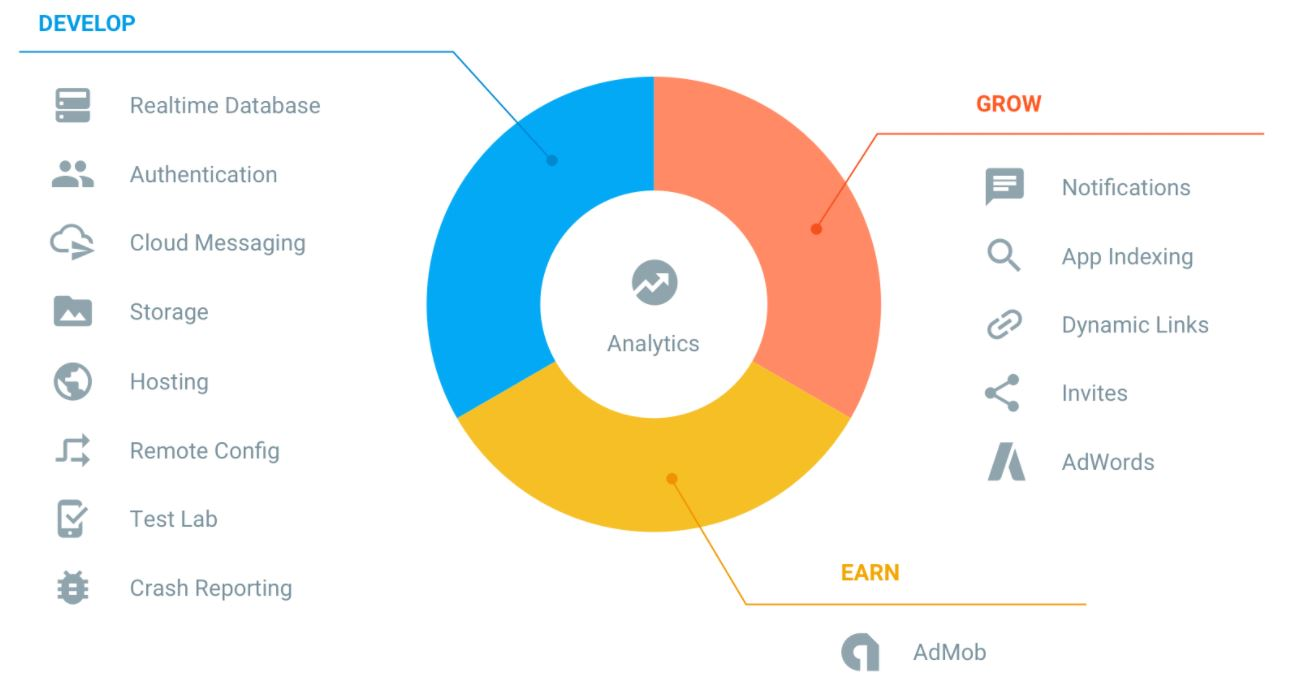
\includegraphics[width=\columnwidth]{../images/firebase.JPG}
	\caption{ Components of Firebase cloud services 
		\cite{hid-sp18-409-www-firebase}}
	\label{fig:firebase}
\end{figure}

\subsection{Development and testing services}

\subsubsection{Realtime Database}
The Firebase Realtime Database is a cloud-hosted, NoSQL database to store and 
sync data between Mobile and web application in realtime. This NoSQL Realtime 
Database is a really big JSON object structure which could be managed in 
realtime~\cite{hid-sp18-409-www-firebase-wikipedia, 
	hid-sp18-409-www-firebase-products}. Firebase database is easily plugable 
	and 
any application could hold current value of the data and any updates to that 
using a single API as data updates syncs across connected devices in 
milliseconds. Highlighted advantages for Realtime Database are serverless app 
support, optimized for offline use, strong user-based security and part of the 
Google echo system~\cite{hid-sp18-409-www-firebase-products}.

\subsubsection{Crashlytics}
Crashlytics is a crash reporting services provided by Firebase technologies to 
reduce troubleshooting time by turning crash reports into a manageable list of 
issues to allow bug fixes in 
realtime~\cite{hid-sp18-409-www-firebase-products}. Crashlytics dashboard 
provides more insights for the developers to identify which issues should be 
prioritized based on user impact. Identified advantages are quickness in 
identifying root cause of crashes, prioritized issues and realtime alerts for 
crashes~\cite{hid-sp18-409-www-firebase-products}. Crashlytics is the successor 
for Firebase Crash Reporting service and currently in beta state.

\subsubsection{Crash Reporting}
Firebase Crash Reporting service is the predecessor for Crashlytics and moving 
to the deprecated state. Pinpointed advantages were easy integration, clustered 
and prioritized errors and version based problem 
identification~\cite{hid-sp18-409-www-firebase-products}.

\subsubsection{Cloud Firestore}
Cloud Firestore is the successor for Firebase Realtime Database service and 
currently in beta state. Firestore is also a cloud-hosted, NoSQL database to 
store and sync data between users at a global scale. Highlighted advantages are 
enhanced query and data structures, enabling truly serverless apps,  syncing 
data across devices, on or offline and scalability 
~\cite{hid-sp18-409-www-firebase-official, hid-sp18-409-www-firebase-products}. 

\subsubsection{Authentication}
Firebase Authentication is an open source authentication service which consist 
of easily plugable SDKs and ready-made user interface libraries to authenticate 
users in iOS, Android and the web applications. Firebase Auth allows different 
methods to authenticate such as email-password, Google, Facebook and Twitter 
using 10 lines of code, including complex operations like account 
merging~\cite{hid-sp18-409-www-firebase-products}. Heavily endorsed attributes 
of the Firebase Auth are flexible, drop-in user interfaces, comprehensive 
security and fast implementation~\cite{hid-sp18-409-www-firebase-wikipedia}.

\subsubsection{Cloud Functions}
Cloud functions enables true server-less applications by deploying a custom 
backend code as a Firebase Cloud function which could be triggered by any 
Firebase product such as Cloud Messaging. Main advantages of Cloud functions 
are server-less application support, low maintenance and enabling high security 
for business logic~\cite{hid-sp18-409-www-firebase-products}.

\subsubsection{Cloud Storage}
Firebase Cloud storage allows developers to store and share application 
generated content such as multimedia items via an object storage in Google 
scale regardless of network quality with high security. Major advantages of 
using Firebase Cloud Storage are scalability at Google scale, robust uploads 
and downloads and strong user-based 
security~\cite{hid-sp18-409-www-firebase-products}.

\subsubsection{Hosting}
Hosting service offers fast and reliable web hosting for modern web 
applications using Solid-state drives(SSDs) inside Content Delivery 
Network(CDN) edge servers all around the world. This service provides free SSL 
certificates for custom domains~\cite{hid-sp18-409-www-firebase, 
	hid-sp18-409-www-firebase-products}.

\subsubsection{Test Lab for Android }
Firebase Test Labs allows developers to utilize large number of mobile test 
devices to test android applications by executing automatic and customized 
tests on virtual and physical devices maintained by Google. Pinpointed 
advantages for Test Lab service are easy integration with existing work flows, 
test any mobile application with zero or minimal coding and availability of 
wide range of devices for beta 
testing~\cite{hid-sp18-409-www-firebase-products}.

\subsubsection{Performance Monitoring}
Performance Monitoring service enables tracing and diagnosing the performance 
of specified components of the mobile application with zero or minimal coding 
effort inside the Firebase console as a detailed or summarized view. Key fact 
about Monitoring service is that it allows to keep the eyes on network behavior 
and pinpoint the origin of issues in mobile 
application~\cite{hid-sp18-409-www-firebase-products}.


\subsection{Audience growing and engaging services}

\subsubsection{Google Analytics}
Google Analytic service is distributed under the Firebase services and it 
allows developers to analyze user behaviours in real-time to do important 
decision making~\cite{hid-sp18-409-www-firebase}. It also allows to export user 
behaviours to Google BigQuery to do advanced analysis. Few important facts of 
Google Analytics are capturing user insights from acquisition to app usage, 
attribution across dozens of sources, segmentation and optimization in one 
dashboard and real-time analytics~\cite{hid-sp18-409-www-firebase-products}.

\subsubsection{Cloud Messaging}
Firebase Cloud Messaging (FCM) is the most used Firebase service among all the 
services as it provides a reliable and energy-efficient messages and push 
notifications on iOS, Android, and the web at no 
cost~\cite{hid-sp18-409-www-firebase-products}. Developer has the control over 
to configure these messages so that it could be sent to a single devices, 
groups of devices, or specific topics or user segments. Advantages associated 
with FCM are advanced message targeting, customizable notification content, 
minimal coding required for configuring or sending notifications, scalability 
up to hundreds of billions of messages per day and A/B test 
notifications~\cite{hid-sp18-409-www-firebase-merged, 
	hid-sp18-409-www-firebase-products}.

\subsubsection{Predictions}
Firebase Prediction services runs on top of Firbase Analytics services to make 
predictions to create dynamic user groups based on different user behaviours 
using Google's machine learning capabilities. Created user groups could be then 
used for sending smart and filtered notifications and messages without worrying 
about different content filtering mechanisms. Highlighted content for 
Prediction services is creating customized user experiences using smarter 
notifications~\cite{hid-sp18-409-www-firebase-products}.

\subsubsection{Dynamic Links}
Dynamic Links allows developers to deliver a customized user experience by 
providing deep links to navigate users to the right place inside iOS, Android, 
and the web application. Few advantages comes with Dynamic Link activation are 
converting mobile web users to native application users, increasing conversion 
for user-to-user sharing, allowing more installs with social, email, and SMS 
marketing campaigns and converting desktop users into mobile application 
users~\cite{hid-sp18-409-www-firebase-wikipedia, 
	hid-sp18-409-www-firebase-products}.

\subsubsection{Remote Config}
Firebase Remote Config service allows developers to customize the look and feel 
of the application for individual users or user groups based on their 
behaviours. It also enables roll out features gradually, run A/B tests and 
customized content filtering without having to deploy and install new version 
of the application~\cite{hid-sp18-409-www-firebase-products}.

\subsubsection{Invites}
Invites service enables in app sharing using referral codes via email or SMS. 
It collaboratively works with Google analytics to provide feedback to the 
developer about invites such as user has opened or installed an application via 
an Invite~\cite{hid-sp18-409-www-firebase-products, 
	hid-sp18-409-www-firebase-invite}.

\subsubsection{App Indexing}
Firebase App Indexing uses Google Search integration to engage users with a 
particular application when searched for related content. If the application is 
already installed, open card will be appeared. If it is not installed, an 
installation card will be shown. Highlighted advantages of using App Indexing 
service are improving your ranking on Search, attraction of new users and 
increasing revenue with better in-app ad 
targeting~\cite{hid-sp18-409-www-firebase-products}.

\subsubsection{AdMob}
Firebase AdMod service allows developers to implement monetization strategies 
inside the application to earn money by showcasing engaging ads to the 
application audience~\cite{hid-sp18-409-www-firebase-admob}.

\subsubsection{AdWords}
Adwords service enables advertisement about the application  sharing across 
Google search to target filtered or not filtered user segments defined inside 
Google Analytics~\cite{hid-sp18-409-www-firebase-adwords}.

\section{Usage}
Firebase could services are trusted by many popular applications such as 
Doodle\cite{hid-sp18-409-www-doodle}, American 
Express\cite{hid-sp18-409-www-americanexpress}, The New York 
Times\cite{hid-sp18-409-www-nytimes}, NPRone\cite{hid-sp18-409-www-npr}, 
Shazam\cite{hid-sp18-409-www-shazam}, Duolingo\cite{hid-sp18-409-www-duolingo}, 
Alibaba\cite{hid-sp18-409-www-alibaba}, Lyft\cite{hid-sp18-409-www-lyft}, 
Venmo\cite{hid-sp18-409-www-venmo}, The 
Economist\cite{hid-sp18-409-www-economist}, 
Trivago\cite{hid-sp18-409-www-trivago}, CTrip\cite{hid-sp18-409-www-ctrip}, 
WattPad\cite{hid-sp18-409-www-wattpad}, KCB\cite{hid-sp18-409-www-kcbgroup}, 
Halfbrick\cite{hid-sp18-409-www-halfbrick}, 
Rockbite\cite{hid-sp18-409-www-rockbitegames}, 
Onefootball\cite{hid-sp18-409-www-onefootball}, 
Fabulous\cite{hid-sp18-409-www-thefabulous} and many 
more~\cite{hid-sp18-409-www-firebase,hid-sp18-409-www-firebase-usecases}. 
According to the Firebase product review reports following applications are 
highlighted to showcase the use cases of Firebase cloud services.
\begin{itemize}
	\item Doodle had increased their user engagement by 42 percent after using 
	Firebase Crashlytics and Remote Config 
	services~\cite{hid-sp18-409-www-doodle, 
		hid-sp18-409-www-firebase-usecases}. 
	
	\item American Express was able to reduce application load testing cost by 
	half after integrating Firebase Test 
	Lab~\cite{hid-sp18-409-www-americanexpress}. 
	
	\item KCB Group was able to reduce the application cost per install by 24 
	percent after utilizing Google Analytics for 
	Firebase~\cite{hid-sp18-409-www-kcbgroup, 
		hid-sp18-409-www-firebase-usecases}.
	
	\item Halfbrick game studio was able to increase 7-day retention rate from 
	25percent to 30 percent after integrating Firebase Predictions with Remote 
	Config to provide in-app promotion to 
	users~\cite{hid-sp18-409-www-halfbrick, hid-sp18-409-www-firebase-usecases}.
	
	\item Rockbite Games development platform was able to boost application 
	revenue up to 25 percent by integrating Firebase Predictions to optimize 
	the digital store user interface for users who were most likely to make an 
	in-app purchases~\cite{hid-sp18-409-www-rockbitegames}.
	
	\item NPR application is integrated Firebase Remote Config, Analytics and 
	BigQuer to gain much smarter targeting and 
	insights~\cite{hid-sp18-409-www-firebase-usecases}.
\end{itemize}

\section{summary}
This paper focused on investigating technical aspects of Firebase cloud 
technologies and its usages. According to the understanding gain from the 
review, it is evident that Firebase cloud technologies has everything needed to 
build and grow Android, iOS, and web applications, all in one place. As James 
\cite{hid-sp18-409-www-firebase}, the founder of Firebase stated, push 
notification support for Android and iOS mobile application is recently 
identified as the most famous feature of Firebase cloud services. Firebase 
cloud services are currently being used by many popular applications and it has 
more than 10 Million active developers on its platform  at the end of 
2016\cite{hid-sp18-409-www-firebase}.

\begin{acks}

  The authors would like to thank Dr.~Gregor~von~Laszewski for his
  support and suggestions to write this paper.

\end{acks}

\bibliographystyle{ACM-Reference-Format}
\bibliography{report} 

